
%%%%%%%%%%%%%%%%%%%%%%%%%% EDP Science %%%%%%%%%%%%%%%%%%%%%%%%%%%%
%
%%%\documentclass[option]{webofc}
%%% "twocolumn" for typesetting an article in two columns format (default one column)
%
\documentclass{webofc}
\usepackage[varg]{txfonts}   % Web of Conferences font
\usepackage{color}
% \usepackage[usenames]{color}
% \usepackage{colortbl}
%
\begin{document}
%
\title{FUMILI-based minimization with constraints using method of elimination of differentials}

\author{
  \firstname{Vladimir} \lastname{Kurbatov},~
  \firstname{Victoria} \lastname{Tokareva}\thanks{
    \email{tokareva@jinr.ru}
   },~
  \firstname{Dmitry} \lastname{Tsirkov}
}

\institute{Laboratory of Nuclear Problems, Joint Institute for Nuclear Research, \\6 Joliot-Curie, Dubna, Moscow region, 141980, Russia}

%TODO: rewrite the abstract a bit different, if possible (the current version has been written for AYSS-18 abstracts and published already)

\abstract{
Some minimization problems, in addition to usual constant limits for single parameters, could imply constraints, i.e. additional relations between parameters $P_1, …, P_n$ in form of equations $\varphi(P_1, \dots, P_n) = 0$.
Often these equations are non-linear and complicated, and thus it is impossible or impractical to eliminate redundant parameters directly. A notable example of such problem is kinematic fitting.
A minimization approach called a method of elimination of differentials is being developed at JINR as an extension to the FUMILI minimizer. It is being used to perform kinematic fitting while analyzing data collected at the ANKE spectrometer.
The talk will cover the mathematical principles of the method, its software implementation and API, and present some examples of its usage.
}
%
\maketitle
   %DONE

% ОБЩИЙ ПЛАН СТАТЬИ
%
% 1 мотивация: кинфит - это очень очень нужно и важно
% 2 кинфит делается посредством минимизации со связями
% 3 история вопроса: два метода
% 4 в ОИЯИ был предложен третий метод - очень кратко суть метода -  как расширение минимизатора ФумилиЁ разработанного так же с ОИЯИ
% 5 минимиатор Фумили хорош тем-то и тем-то (по сравнению с аналогами)
% 6 метод со связями хорош тем-то и тем-то
% 7 программная реализацияЁ как и почему
% 8 пример игрушечный
% 9 пример настоящий
% 10 планы и заключение - "спасти человечество"Ё не меньше))
% 11 библиография

% Фитирование - это настройка весов вычислительной модели таким образом, чтобы она максимально удовлетворяла реальным данным, полученным в эксперименте.
% При этом чем больше мы имеем данных о физике происходящего процесса, тем более адекватные значения параметров мы сможем поулчить в результате подгонки.
% Эти данные, будучи выражены в форме уравнений типа ``кракозябра = 0'', называются связями (constraints).
% Использование такой, более точной, аппроксимации востребовано во многих областях физики. Одной из таких областей является кинематическ


\section{Kinematic fitting}
% Распространенной ситуацией в ФЭЧ является выяснение параметров вычислительной модели путем фитирования экспериментальных данных. Как правило, вычисления подобных зависимостей являются достаточно тяжёлыми и не точными, поскольку размерность уравнений, как правило, является очень высокой. Для снижения размерности уравнений мы можем использовать данные о кинематике реакции, выраженные в форме уравнений связи.
%
% Например, могут быть использованы закон сохранения массы или инвариант Лоренца.
%
% В общем случае данные о кинематике реакции могут быть записаны in form of equations \eqref{eq:constr}:
% \begin{equation}
% \label{eq:constr}
% \left\{
% \begin{aligned}
% \phi_1(P) &= 0,\\
% \cdots\\
% \phi_n(P) &= 0,
% \end{aligned}
% \right.
% \end{equation}
% where $P$ is a vector of parameters.
% в большинстве случаев данные уравнения связи являются нелинейными и сложными, и сокращение размерности системы \eqref{eq:constr} путем непосредственного решения оказывается невозможным или не имеющим смысла.

The problem of track reconstruction is generally a problem of multidimensional linear regression: for each of the tracks $j$ we need to find such initial momenta $\boldsymbol{p}^j$ that the reconstructed coordinates of detector hits $\hat{c}_i^j(\boldsymbol{p}^j)$, where $i$ is a hit number, would be a close a possible to the registered hit coordinates $c_i^j$, taking into account the known detector uncertainties $\delta c_{i^j}$.
% Задача восстановления трека частицы (фитирования) в общем случае представляет собой задачу многомерной линейной реграссии: для каждого из треков $j$ требуется найти изначальные импульсы $P^j$, такие, чтобы теоретически вычислимое положение точек трека $\hat{c}_i^j(P^j)$, где $i$ - номер координаты точки, максимально приближалось к фактическому распределению точек $c_i^j$, при этом учитывая известные ошибки детектора $\delta c_{i^j}$.
The actual problem we are solving is the minimization problem for the functional
% Фактически, решается задача минимизации функционала:
\begin{equation}
\label{track_fit}
F(\boldsymbol{p}^j, c_i^j) = \sum_i \left(\frac{c_i^j - \hat{c}_i^j(\boldsymbol{p}^j)}{\delta c_i^j}\right)^2.
\end{equation}
Further we would omit the indices $i$, $j$ for simplicity, so that $\boldsymbol{c}$ and $\boldsymbol{p}$ would be the vectors of all hits and momentum components correspondingly.
% Здесь и далее для простоты будем опускать коэффициенты $i,~j$.

Often we could get the additional information in reaction kinematics in the form of energy-momentum conservation laws
% Зачастую известна дополнительная информация о кинематике реакции в виде законов сохранения энергии и импульса
\begin{equation}
\label{cons_full}
\sum\mathcal{P}_\mathrm{initial} = \sum\mathcal{P}_\mathrm{final}
\end{equation}
or, when one of the final particles is not registered,
\begin{equation}
\label{cons_miss}
\displaystyle\left|\sum\mathcal{P}_\mathrm{initial} - \sum\mathcal{P}_\mathrm{final}\right|^2 = M_X^2,
\end{equation}
where $\mathcal{P}$ is the four-momentum of a particle, and $M_X$ is the reaction missing mass.

Using them allows to narrow down the multidimensional domain of this functional and improves the precision of the solution.
% Её использование позволяет сузить многомерную область определения данного функционала и положительно влияет на точность получаемого решения.
The fitting that takes these conditions into account is called kinematic.
It is widely employed in high energy physics, e.g.\ in experiments like 
% Выполняемый с учётом данных условий фит называется кинематическим и находит широкое применение в ФЭЧ, например, в таких экспериментах как
BES-III, % http://iopscience.iop.org/article/10.1088/1674-1137/34/2/009/meta
CLAS, % https://scholar.google.ru/scholar?cites=6441758058779809394&as_sdt=2005&sciodt=0,5&hl=ru
CMS. % http://cds.cern.ch/record/926540

In this paper we are going to cover the development of a Fumili-based framework for kinematic fitting that is currently used by the authors for kinematic fitting in the ANKE experiment (Jülich, Germany)~\cite{anke}.
% В данной статье мы собираемся рассказать об опыте разработки Fumili-based фреймвока для кинематического фита, в настоящий момент применяемого авторами для кинематического фита в эксперименте ANKE (Jülich, Germany)~\cite{anke}.

\section{Constrained minimization}
% The problem of minimizing functionals with constraints arises, for example, in the task of kinematic fitting.
% % \begin{block}{Kinematic fitting}
% \begin{itemize}
% \item Tracking detectors provide the coordinates of the triggered sensitive elements along with their errors;
% \item Track-finding involves fitting the particle trajectories to these coordinates;
% \item Sometimes, when the reaction channel is known, the additional information on kinematics could be utilized in terms of
% % \begin{description}
% \item[conservation laws:] $\sum E_\mathrm{initial} = \sum E_\mathrm{final}$, $\displaystyle\sum\vec{P}_\mathrm{initial} = \sum\vec{P}_\mathrm{final}$;
% \item[missing mass:] $\displaystyle\left|\sum\boldsymbol{P}^{(4)}_\mathrm{initial} - \sum\boldsymbol{P}^{(4)}_\mathrm{final}\right|^2 = M_X^2$;
% \end{itemize}
%
% % \end{description}
% This is called \emph{kinematic fitting}.

% The minimum search for the functional \eqref{track_fit} could be formulated as a conditional-minimization problem in canonical form, 
% taking into account the known 

The conservation laws (\ref{cons_full}--\ref{cons_miss}), could be expressed as
% Поставленная задача нахождения минимума функционала \eqref{track_fit} может быть сформулирована как задача условной минимизации в канонической форме, с учетом известных законов сохранения \eqref{cons_full}--\eqref{cons_miss}, выраженных в виде:
\begin{equation}
\label{eq:constr}
\phi_k(\boldsymbol{p}) = 0, 1 \leqslant k  \leqslant m,
\end{equation}
where $m$ is a number of constraints.

Then \eqref{track_fit}, \eqref{eq:constr} is a constraint minimization problem written into the augmented form.

The cases of interest is those where the system \eqref{track_fit},~\eqref{eq:constr} is non-linear and could not be practically solved in a straingh forward way, with taking in account practical time and memory limitations. % в условиях заданных внешних ораничений?
% Предмет интереса представляют случаи, когда система \eqref{eq:constr} является нелинейной и её решение ``в лоб'' является невозможным либо нецелесообразным в условиях заданных внешних ораничений.
% So we need not to lose important information and make calculations as accurately as possible, at the same time keeping within the limitations of time and computational intensity of the work.
% Возникает необходимость не потерять важную информацию и провести расчёты максимально точно, при этом уложившись в ограничения по времени и трудоемкости работы.

% Отличительной особенностью задач кинематического фита, как задачи минимизации со связями является то, что функционал (1) здесь зависит не просто от параметров, но от функции этих параметров.
% The distinctive feature of the kinematic fitting problems is that the functional \eqref{track_fit} here depends not only on parameters $\boldsymbol{p}$, but on the function $\hat{c}(\boldsymbol{p})$.

% \section{Methods}
% % constrMinIntro.tex
% The problem of minimizing functionals with constraints~\eqref{eq:constr} arises, for example, in the task of kinematic fitting. This problem traces back to early sixties, when first solutions for the problem were proposed~\cite{b1,b2}.
% Первые решения в области минимизации со связями в задачах кинематического фита были предложены в начала 60-х. Классическим, до сих пор широко применимым методом здесь является метод множителей Лагранжа (ссылка), который используется, например в (ссылка). Специалистами ОИЯИ (ссылка) примерно в те же годы было предложено применение минимизации с использованием штрафных функций.
% Подход, предложенный одним из авторов доклада в 90-е (ссылка) [очень крутой - TODO: прописать, почему.]

% Первые идеи по преодолению подобных сложностей в задачах кинематического фита были предложены в 60-е.
The first ideas on overcoming such complexities in the problems of kinematic fitting were proposed in the sixties.
% Солмицом и Бёрджем \cite{b1} было предложено применение метода множителей Лагранжа (см. далее), который до сих пор находит широкое применение в задачах подобного типа \cite{b4}. %сюда же можно ещё ссылки на эксперименты, там тоже сплошнй Лагранж
Solmitz and Berge in~\cite{b1} proposed to use the method of Lagrange multipliers (see below), which is still widely used in problems of this type~\cite{b4}. % here you can refer to more experiments, they are also using solid Lagrange
% Примерно в то же время специалистами ОИЯИ было предложено применение минимизации с тяжёлым членом \cite{b5} (будет описано далее) и разработан пакет для минимизации $\chi^2$-функционалов FUMILI~\cite{fum_1st}.
Approximately at the same time JINR specialists proposed the use of minimization with the penalty function~\cite{b5}, described below, and developed a package for minimizing the $\chi^2$-like functionals FUMILI~\cite{fum_1st}.
% Позже, одним из соавторов данной работы, было предложено \cite{b6} использование метода устранения производных для кинфита со связями.
Later, one of the co-authors of this work suggested the method of elimination of differentials for kinematic fitting with constraints~\cite{b6}.

%   \subsection{Method of Lagrange multipliers}
%   % Method of Lagrange multipliers

\begin{itemize}
\item First proposed at early sixties, see e.\,g.\ J.\,P.~Berge, F.\,T.~Solmitz, H.\,D.~Taft, Rev.\ Sci.\ Instr.\ 32 (1961) 538;
\item Uses \emph{Lagrange multipliers} $\lambda_i$, obtained from the equations
\[\frac{\partial\Psi}{\partial x_1} = \frac{\partial\Psi}{\partial x_2} = \cdots = \frac{\partial\Psi}{\partial x_n} = 0,\]
where $\displaystyle\Psi(x) = F(x) + \sum_{i=1}^m\lambda_i\phi_i(x);$
\item Still the most widely used method for kinematic fitting, see e.\,g.\ KWFIT package \texttt{http://www.phys.ufl.edu/\textasciitilde{}avery/kwfit/}.
\end{itemize}

%   \subsection{Penalty function method}
%   % % Penalty-function method}
% \begin{itemize}
% \item Proposed in JINR in mid-sixties, see V.I. Moroz, JINR communications R-1958 (1965);
% \item Adds a so-called ``heavy term'' to the minimized functional, designed in a way that values of constraint functions approach zero as this term approaches infinity:
% \[
% \tilde{\Psi}(x) = F(x) + T\sum_{i=1}^{m}\phi_i^2(x),~T \rightarrow \infty.
% \]
% \item The method is very robust and almost always converges, which could be both a benefit (you won't miss a minimum) and a drawback (you should carefully control that your minimum is reasonable).
% \end{itemize}

%
The method of kinematic fitting employing a ``heavy term'', proposed by Moroz~\cite{b5}, is based on the method of penalty functions for solving conditional optimization problems.
% Метод кинематического фита с тяжелым членом, предложенный В.И.Морозом, основан на методе штрафных функций решения задач условной оптимизации.

The essence of the method is to reduce the task of minimizing the function \eqref{track_fit} with the conditions \eqref{eq:constr} to the problem of finding the unconditional minimum of the function
% Суть метода состоит в сведении задачи минимизации функции \eqref{track_fit} при выполнении условий \eqref{eq:constr} к задаче поиска безусловного минимума функции
\begin{equation}
\hat{F}(\boldsymbol{p}, \boldsymbol{c}) = F(\boldsymbol{p}, \boldsymbol{c}) + T\sum_{k=1}^{m}\phi_k^2(\boldsymbol{p}),~T \rightarrow \infty.
\end{equation}

% При этом функцию $\tilde{\Psi}(P, c)$ называют штрафной или функцией с тяжёлым членом $T$.
In this case, the function $\hat{F}(\boldsymbol{p}, \boldsymbol{c})$ is called a penalty function or a function with a ``heavy term'' $\displaystyle T\sum_{k=1}^{m}\phi_k^2(\boldsymbol{p})$.
% При такой постановке при выходе за пределы, задаваемые ограничениями \eqref{eq:constr}, слагаемое ``с тяжёлыми членом'' будет увеличивать значение минимизируемой функции, таким образом гарантируя, что оптимальное значение может быть найдено только в пределах области ограничений.
With this formulation of the problem, if we exceed the limits specified by the constraints \eqref{eq:constr}, the ``heavy term'' will increase the value of the minimized functional, thus ensuring that the optimal value can be found only within the constraint area.

% Минимизация штрафной функции может выполняться с использованием любого метода оптимизации, например, градиентного спуска.
The minimization of the penalty function can be performed using any optimization method, for example, gradient descent.

  \subsection{Method of elimination of differentials}
  \textcolor{red}{TODO: привести к общему знаменателю обозначения в формуле с обозначениями в остальной статье!!!}

% обозначим через $np$ число параметров, от которых зависит функционал \eqref{track_fit}, $nc$ - xbckj
В близи фиксированной точки $P_0$ функционал \eqref{track_fit} может быть представлен степенным рядом
% In the neighborhood of a point $x_0$ the functional $F(x)$ could be expressed as
\begin{equation}\label{func_diff}
\begin{aligned}
F(P_0+\Delta P) &= F(P_0) + \sum_{i=1}^n \frac{\partial F(P_0)}{\partial P_i} \Delta P_i + \frac{1}{2}\sum_{i=1}^n\sum_{j=1}^n \Delta P_i \frac{\partial^2 F(P_0)}{\partial P_i \partial P_j} \Delta P_j\\
&= F(P_0) + G(P_0) \Delta P + \frac{1}{2}\Delta P^T Z(P_0) \Delta P,
\end{aligned}
\end{equation}
Данную формулу можно переписать в матричном виде как:

\begin{equation}
 \label{eq_diff1}
x^2
\end{equation}


and the constraints $\Phi(x)$ as
\begin{equation}\label{constr_diff}
\Phi(x_0+\Delta x) =
\left[
\begin{aligned}
\phi_1(x_0) +& \sum_{i=1}^n \frac{\partial \phi_1(x_0)}{\partial x_i}\Delta x_i\\
&\cdots\\
\phi_m(x_0) +& \sum_{i=1}^n \frac{\partial \phi_m(x_0)}{\partial x_i}\Delta x_i\\
\end{aligned}
\right]
= \Phi(x_0) + D(x_0) \Delta x.
\end{equation}

In the matrix equation $\Phi(x) = \Phi(x_0) + D(x_0) \Delta x$ the rectangular matrix $D$ has $m$ rows and $n$ columns (we have $n$ parameters and $m$ constraints).

The vector $\Delta x$ could be split into $\Delta x_c$ that has $m$ components, and $\Delta x_f$ that has $n-m$ components; the same could be done with the matrix $D$. Then
\begin{equation}\label{phi_split}
\Phi(x) = \Phi(x_0) + D_c(x_0) \Delta x_c + D_f(x_0) \Delta x_f.
\end{equation}
Since \eqref{phi_split} is a linear equation, it could be solved in relation to $\Delta x_c$, resulting in
\begin{equation}\label{X_c}
\Delta x_c = \mathbf{v} + M \Delta x_f.
\end{equation}
Returning to the initial functional \eqref{func_diff}
\[F(x) = F(x_0) + G(x_0) \Delta x + \frac{1}{2}\Delta x^T Z(x_0) \Delta x,\]
we could employ \eqref{X_c} to eliminate the sub-vector $\Delta x_c$, and obtain a similar functional, in contrast depending on only $n-m$ increments $\Delta x_f$:
\begin{equation}\label{func_fin}
F(x) = F'(x_0) + G'(x_0) \Delta x_f + \frac{1}{2}\Delta x_f^T Z'(x_0) \Delta x_f.
\end{equation}

\section{Fumili-based realization of the method}
% \textcolor{red}{Some words about Fumili and its advantages.}
% 
FUMILI is one of the first minimizers included into ROOT release.
It has been showing it's reliability, stability and high convergence rate while it had been being used by scientific community for decades.

The greedy minimization algorithm which is employed in FUMILI was first proposed and developed at JINR by I.\,N.~Silin and V.\,S.~Kurbatov.

FUMILI provides an optimal solution for $\chi^2$-like functionals \eqref{xisq_func} employing linearization:
\begin{equation}
\label{xisq_func}
F(\boldsymbol{p}) = \sum_{k=1}^K f_k^2(\boldsymbol{p}) = \sum_{k=1}^K\left(\frac{c_k - \hat{c}_k(\boldsymbol{p})}{\delta c_k} \right)^2,
\end{equation}
where $c_k$ are measured values with errors $\delta c_k$, $k \in [1, K]$, and $\hat{c}_k(\boldsymbol{p})$ are the values predicted by the model, depending on some parameters $\boldsymbol{p} = \{p_1, \ldots, p_n\}$.

% {Linearization method in minimizing $\chi^2$-like functionals}
The second derivative $\displaystyle\frac{\partial^2 F}{\partial p_i p_j}$ could be found the following way:
\begin{equation}
\begin{aligned}
%  \label{linear}
\frac{\partial^2 F}{\partial p_i \partial p_j} &= \frac{\partial}{\partial p_i}\frac{\partial}{\partial p_j} \sum_{k=1}^K f_k^2(\boldsymbol{p}) = \frac{\partial}{\partial p_i}\sum_{k=1}^K 2 f_k(\boldsymbol{p}) \frac{\partial f_k(\boldsymbol{p})}{\partial p_j} = \\
&= 2 \sum_{k=1}^K \left( \frac{\partial f_k(\boldsymbol{p})}{\partial p_i}\frac{\partial f_k(\boldsymbol{p})}{\partial p_j} + f_k(\boldsymbol{p}) \frac{\partial^2 f_k(\boldsymbol{p})}{\partial p_i \partial p_j} \right)
\end{aligned}
\end{equation}
\emph{Linearization} means discarding the second term $\displaystyle f_k(\boldsymbol{p})\frac{\partial^2 f_k(\boldsymbol{p})}{\partial p_i \partial p_j}$ employing second derivatives, that is considered small in comparison to the first one $\displaystyle\frac{\partial f_k(\boldsymbol{p})}{\partial p_i}\frac{\partial f_k(\boldsymbol{p})}{\partial p_j}$.

Its main benefit is that the error matrix for a linearized functional is always positively defined, and thus each step leads to a minimum.


% \textcolor{red}{What do we need to write about implementation?}
%   программная реализация будет здесь же
%programming realization

\textcolor{red}{
TODO: There must be an explanation of why we include it specifically in Fumili.
Well, or it should appear in the previous part, where we've spoken about Fumili.
}

%очень общая схема включения дополнения в Fumili и ROOT
% \centering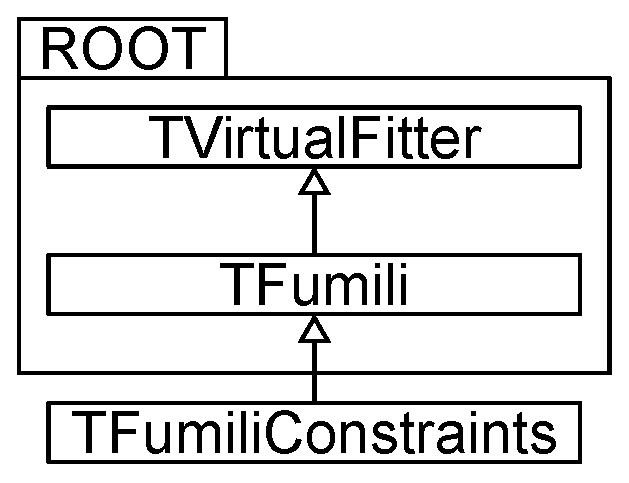
\includegraphics[width=0.4\textwidth]{pics/arch1.eps}

% \begin{figure}[htbp]
% \centering
% \centering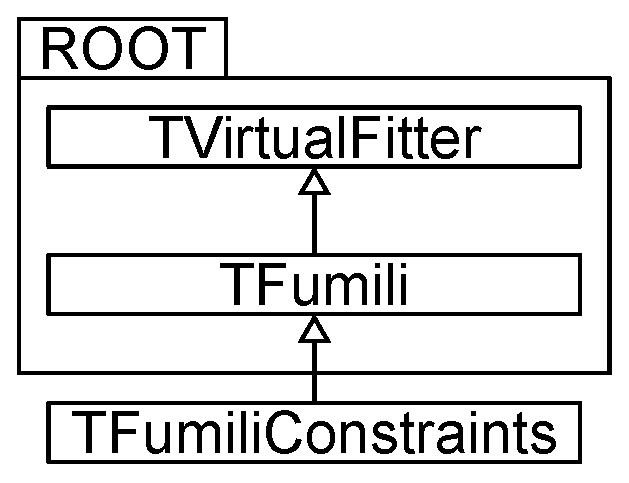
\includegraphics[width=0.35\textwidth]{pics/arch1.eps}
% \caption{
% Схема отношений классов при фитировании.
% Разработанный авторами класс TFumiliConstraints наследует от класса TFumili.
% }
% \label{arch}
% \end{figure}

%фактический user API. Несколько избыточен для статьи и вообще недоработан
% \begin{verbatim}
% void FCN(int & n_par, double * grad,
%          double & val, double * par, int flag);
% /* ... */
% TFumiliConstraints * fum = new TFumiliConstraints;
% // set parameters
% fum->SetParNumber(2);
% fum->SetParameter(0, "#alpha", .5, 0.01, 0, 0);
% fum->SetParameter(1, "#beta", .0, 0.01, 0, 0);
% // set constraints
% fum->SetConstrNumber(1);
% fum->SetConstraint(0, [](double * p){
%   return p[0]*p[0] + .5*p[1] - 1.3;
% });
% fum->SetConstrDeriv(0, 0, [](double * p){ return 2*p[0]; });
% fum->SetConstrDeriv(0, 1, .5);
% // set objective function
% fum->SetFCN(FCN);
% // minimize
% fum->Minimize();
%
% \end{verbatim}


\section{Example: Monte-Carlo simulation}
The algorithm implementation was tested on a simulated set of events.
For this purpose 500\,000 $(a,b)$ events were Monte-Carlo generated according to the function
\begin{equation}
\label{eq:simul}
1 + x_1a + x_2a^2 + x_3b + x_4b^2
\end{equation}
with the parameters
\{$x_1 = 0.5$, $x_2 = 0.3$, $x_3 = 0.8$, $x_4 = 0.1$\}.
Then the same equation \eqref{eq:simul} was fitted to them using an event-by-event log.\ likelihood method with constraints
\begin{equation}
\label{eq:simul:constr}
x_1^2 + x_1x_4 - x_4^2 = 0.29,~x_2^2/x_3 = 0.1125.
\end{equation}

% Results:
% \begin{figure}[htbp]\centering
% 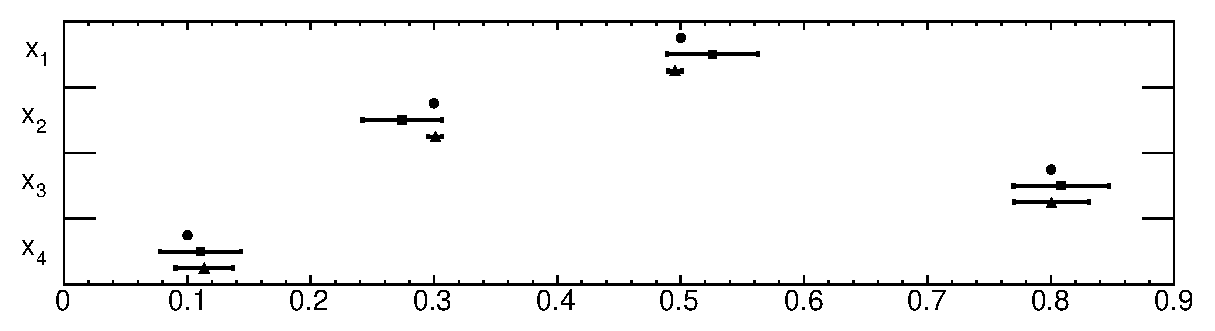
\includegraphics[width=1\textwidth]{pics/drawToyBW.eps}
% \caption{
% The parameter values obtained by fitting the set of events generated according to the equation \eqref{eq:simul}.
% Circles correspond to the original values used in the simulation, squares show the results provided by the fit without constraints, triangles come from the fit with constraints \eqref{eq:simul:constr}.
% }
% \label{toy_errs}
% \end{figure}

\begin{table}[htbp]
\caption{
The parameter values obtained by fitting the set of events generated according to equation \eqref{eq:simul}, with their errors.
}
\label{tab:1}
\begin{tabular*}{1\textwidth}{@{\hspace{2em}}c@{\extracolsep{\fill}}ccc@{\hspace{2em}}}\hline\hline
Parameter & True values & Unconstrained fit & Constrained fit \\\hline
$x_1$ & $0.5$ & $0.526 \pm 0.037$ & $0.496 \pm 0.006$ \\
$x_2$ & $0.3$ & $0.274 \pm 0.032$ & $0.301 \pm 0.006$ \\
$x_3$ & $0.8$ & $0.808 \pm 0.039$ & $0.801 \pm 0.030$ \\
$x_4$ & $0.1$ & $0.111 \pm 0.033$ & $0.114 \pm 0.023$ \\\hline\hline
\end{tabular*}
\end{table}

The results of the fit are presented in
% fig.~\ref{toy_errs} and
table~\ref{tab:1}. They show that constraints could lead to significant improvement in fit precision, that is particularly pronounced in the present case for the parameters $x_2$ and $x_3$.

\section{Kinematic fitting at ANKE}
% Kinematic fitting at ANKE
% Разработанное расширение было использовано авторами для кинематического фита в реакциях $pp \to pp$ и $pp \to pp\pi^0$ на данных, полученных на спектрометре ANKE (Jülich, Germany)~\cite{anke}.
The developed Fumili extension was used by the authors to perform the kinematic fitting of the data obtained at the ANKE spectrometer (Jülich, Germany)~\cite{anke} for the $pp \to pp$ and $pp \to pp\pi^0$ reactions.

% На рисунке \eqref{anke_scheme} можно видеть, что в процессе прохождения протонного пучка через установку часть протонов может отклоняться от направления основного пучка и не фиксироваться установкой, таким образом при анализе данных эксперимента мы можем столкнуться с разницей зафиксированных энергий и количества вещества, вступившего в реакцию с данными, полученными на выходе. Восстановить долю таких ``потерянных'' протонов мы можем, используя инвариант Лоренца $\left|\boldsymbol{P}^{(4)}_\mathrm{beam}+\boldsymbol{P}^{(4)}_\mathrm{targ}-\boldsymbol{P}^{(4)}_p\right|^2 = m_p^2$.

\begin{figure}[htbp]\centering
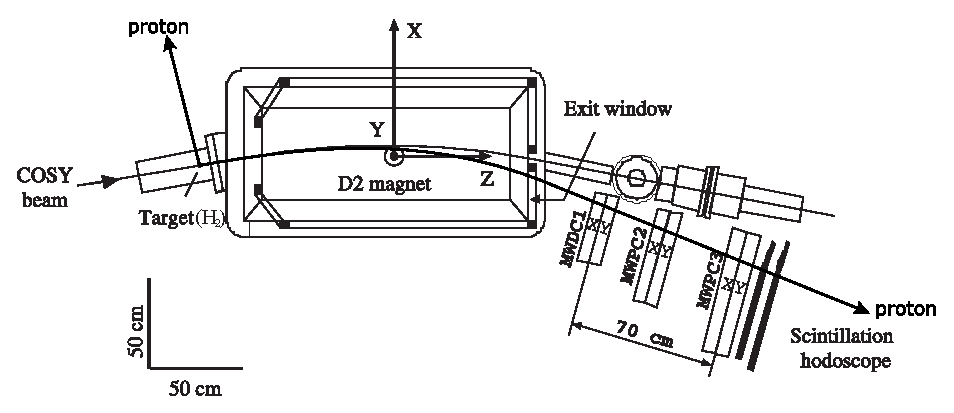
\includegraphics[width=0.8\textwidth]{pics/setup_bw.eps}
\caption{
A scheme of the $pp \to pp$ reaction being registered in the ANKE forward detector. Other ANKE detectors are not shown.
}
\label{anke_scheme}
\end{figure}

\begin{figure}[htbp]\centering
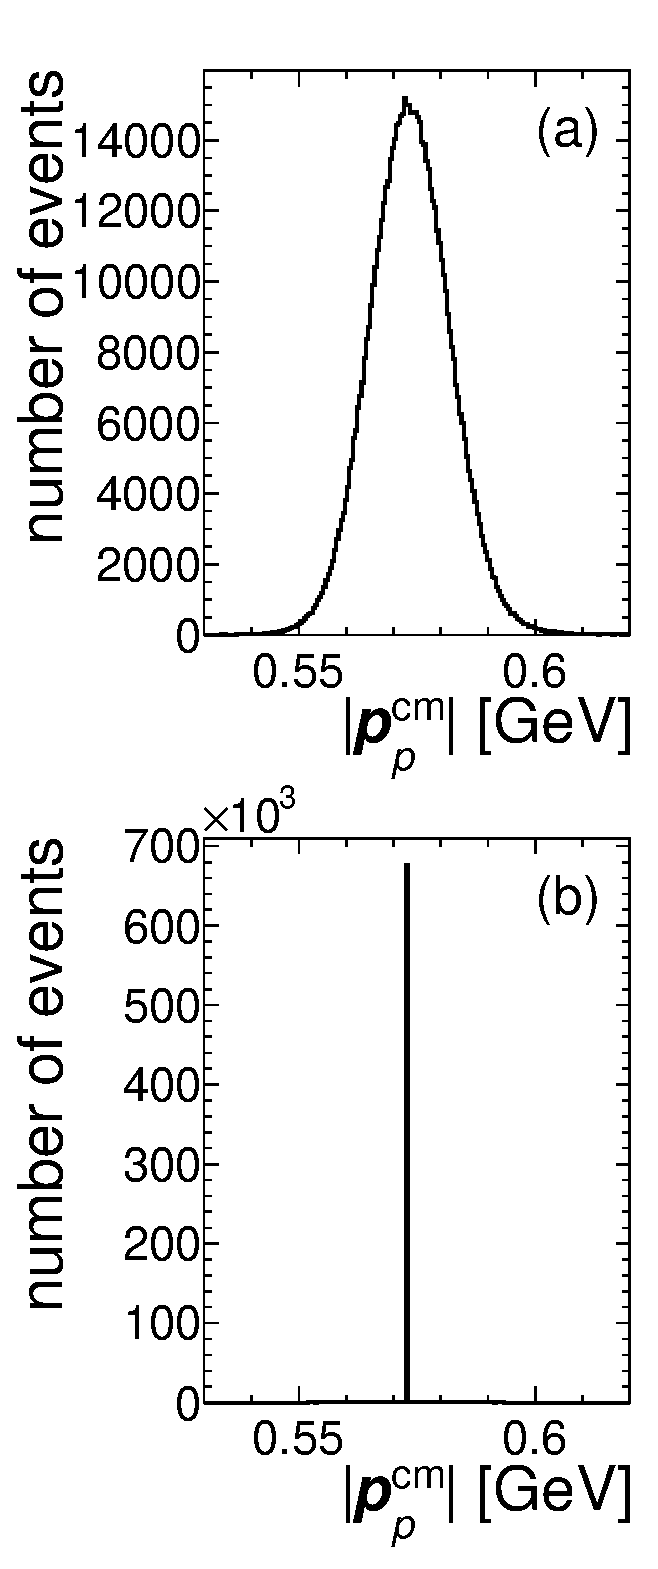
\includegraphics[height=0.3\textheight]{pics/drawMom.eps}
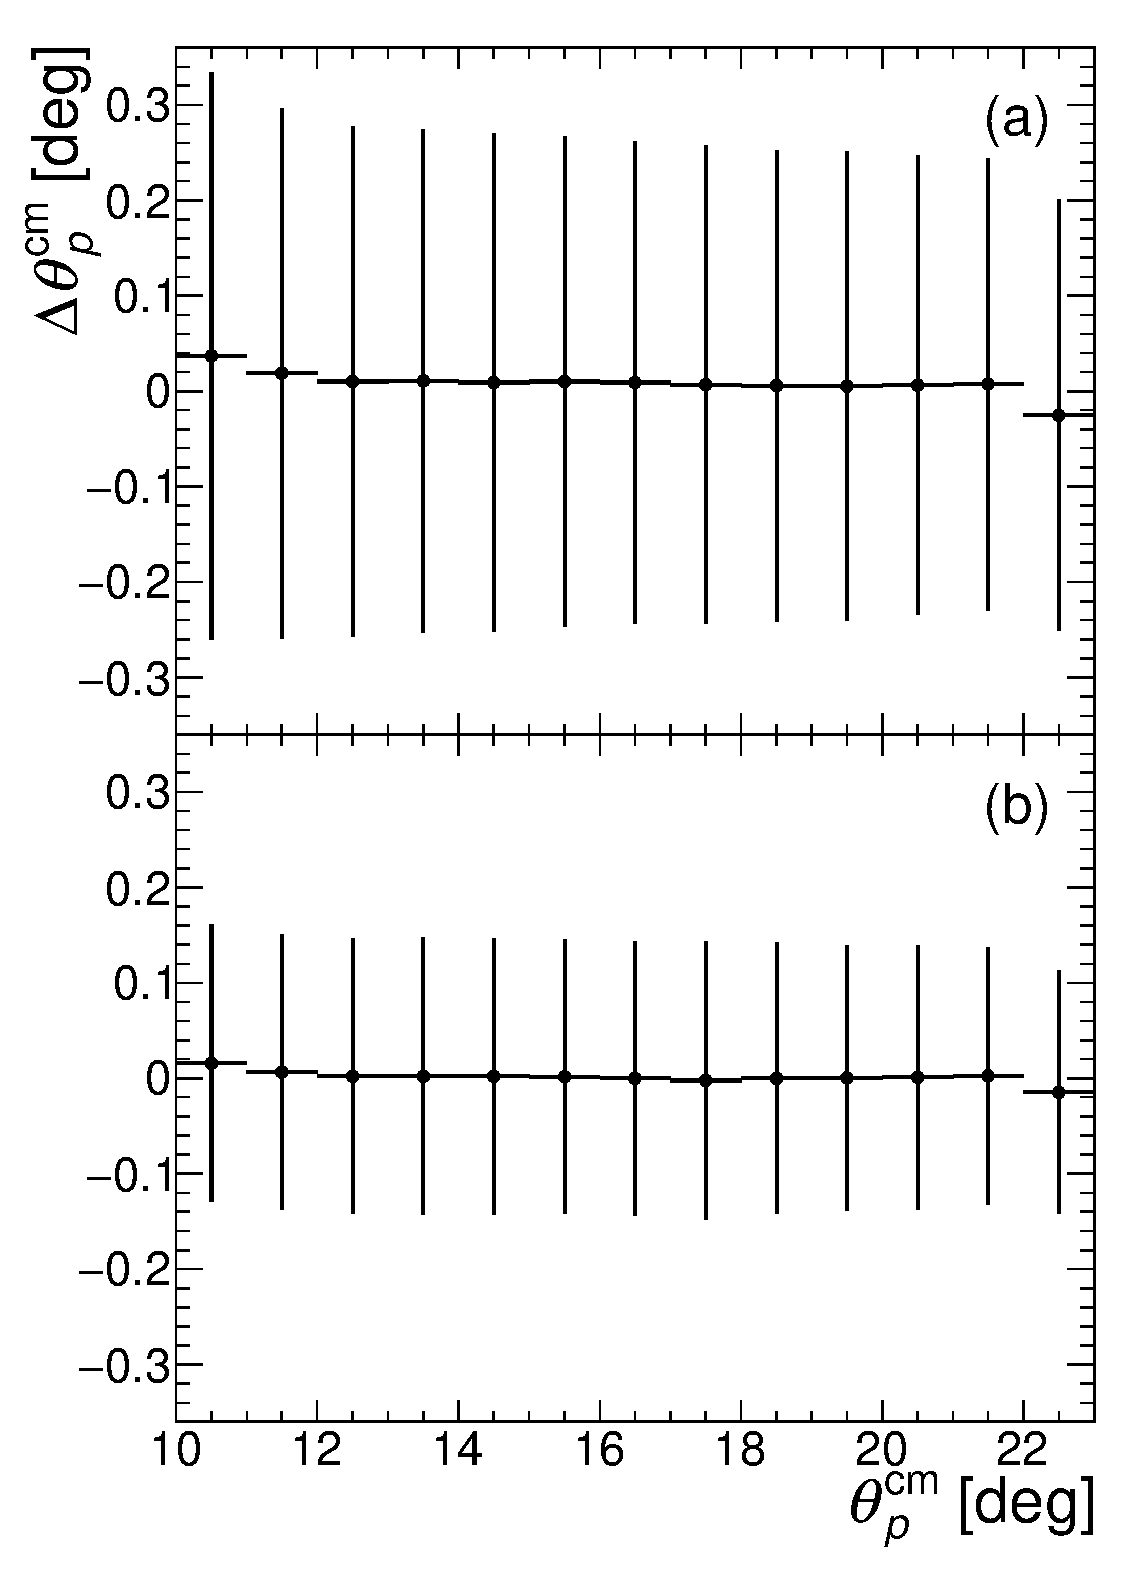
\includegraphics[height=0.3\textheight]{pics/drawTh.eps}
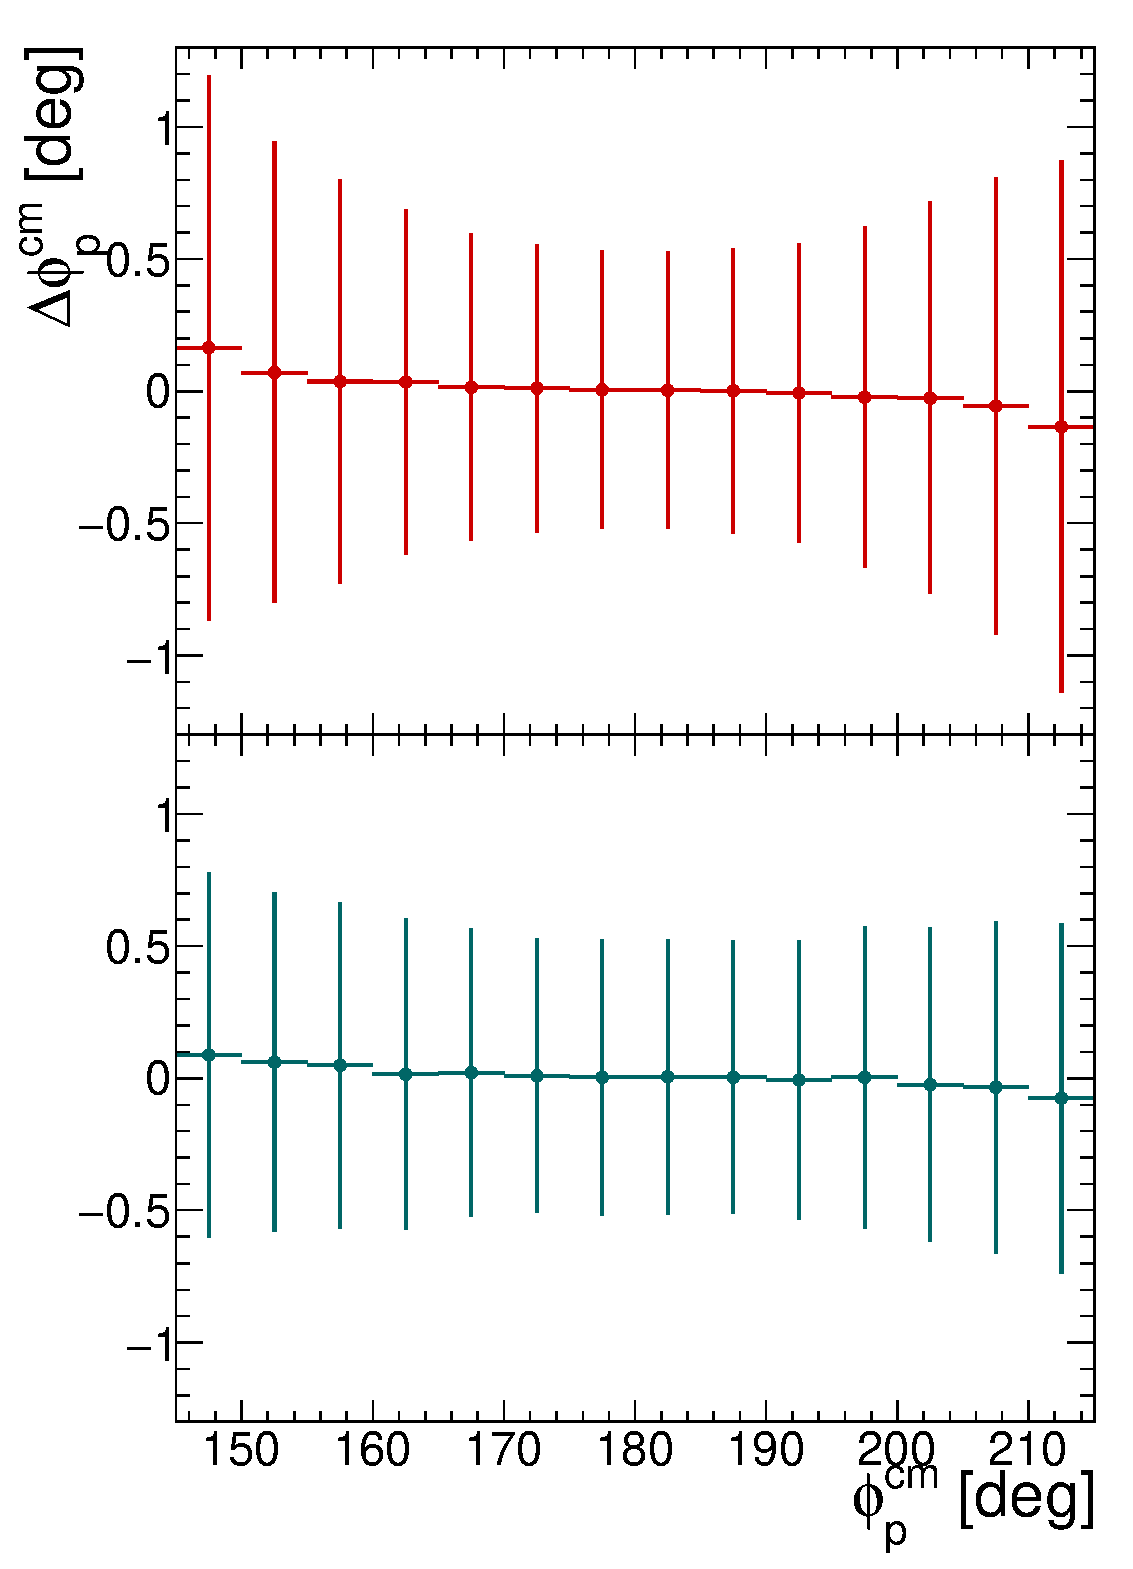
\includegraphics[height=0.3\textheight]{pics/drawPhi.eps}
\caption{
Errors of reconstructed proton momentum in polar coordinates $(|\boldsymbol{p}_p^\mathrm{cm}|, \theta_p^\mathrm{cm}, \phi_p^\mathrm{cm})$ for the $pp \to pp$ reaction at ANKE, simulated for $T_\mathrm{beam} = 700$~MeV either with (a) or without (b) kinematic fitting.
}
\label{anke_errs}
\end{figure}

Let us consider the $pp \to pp$ reaction registered in the forward detector (fig.~\ref{anke_scheme}).
In this case the detector acceptance allows to register only one of the final protons, so we use equation \eqref{cons_miss} for missing mass as a constraint.
Tracking is being done in the forward detector by three multiwire gas chambers, each consisting of several multiwire planes.
A set of signals produced by adjacent wires when a particle passes nearby is called a cluster.
So, an event would contain a set of cluster coordinates $\{c_1, \ldots, c_K\}$ with their errors $\{\delta c_1, \ldots, \delta c_K\}$, and the minimized functional is defined by equation \eqref{track_fit}.
For the study under consideration, the reconstructed coordinates $\hat{c}_k$ are calculated on the basis of the known field map of the analyzing magnet using the Runge–Kutta method, assuming that these particles originated from a point-like source at the center of the target-beam interaction volume.

% Рассмотрим область мишени, изображённую на рис.~\ref{anke_scheme}, где происходит упругое $pp$ взаимодействие и один из протонов регистрируется в координатных камерах Fd.
% Результатом является набор измеренных значений координат кластеров ${C_i:m }$ c ошибками ${\delta C_i}$.

% Истинная координата трека $C_i$ есть функция $C_i = C_i (V, P)$, где вектора $V, P$ содержат координаты вершины и компоненты импульса. Далее делается разумное предположение, что разность $C_i - C_i^m$ распределена по Гауссу с ошибкой ${\delta C_i}$. Функция правдоподобия совокупности измеренных координат
% \begin{equation}
% \label{FPC}
% L_c \approx \prod_i \exp \left(\frac{-1}{2} \left(\frac{C_i - C_i^m}{\delta_{C_i}} \right)^2 \right) \ldotp \Delta C_i
% \end{equation}

% Функция правдоподобия для координат вершины (в предположении, что по каждой координате распределение Гауссово и они независимы; на самом деле функция плотности вероятности распределения по координатам вершины может иметь более сложный вид):
% \begin{equation}
% \label{FPV}
% L_c \approx \prod_i \exp \left(\frac{-1}{2} \left(\frac{V_i - V_i^m}{\delta_{V_i}} \right)^2 \right) \ldotp \Delta V_i
% \end{equation}

% Тогда совместная функция правдоподобия $L_G$ будет иметь вид:
% \begin{equation}
% \label{FPG}
% L_G = L_V \ldotp L_C
% \end{equation}
% Наиболее точная оценка параметров будет получена путём минимизации общей функции правдоподобия $L_G$, однако, если нет информации об $L_V$, оценка параметров производится
% только по $L_C$.

% TODO: Добавить, причем тут Polar CMS coordinates.

% \centering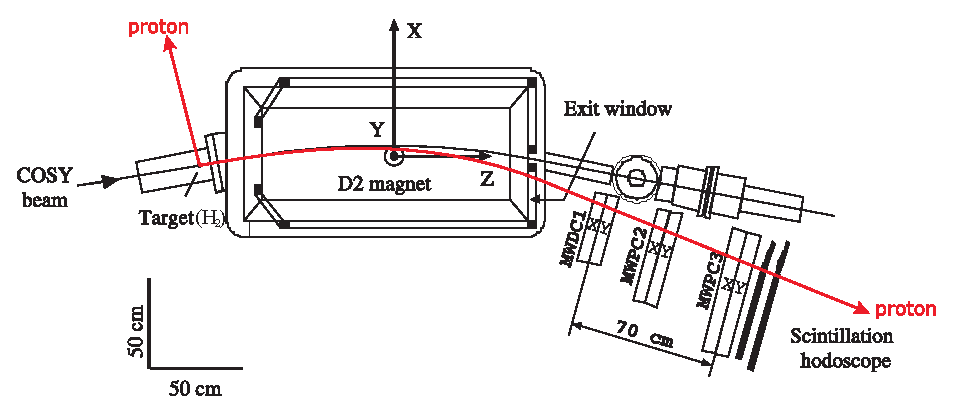
\includegraphics[width=0.8\textwidth]{pics/setup_.eps}

% \large
% \phantom{0}
% 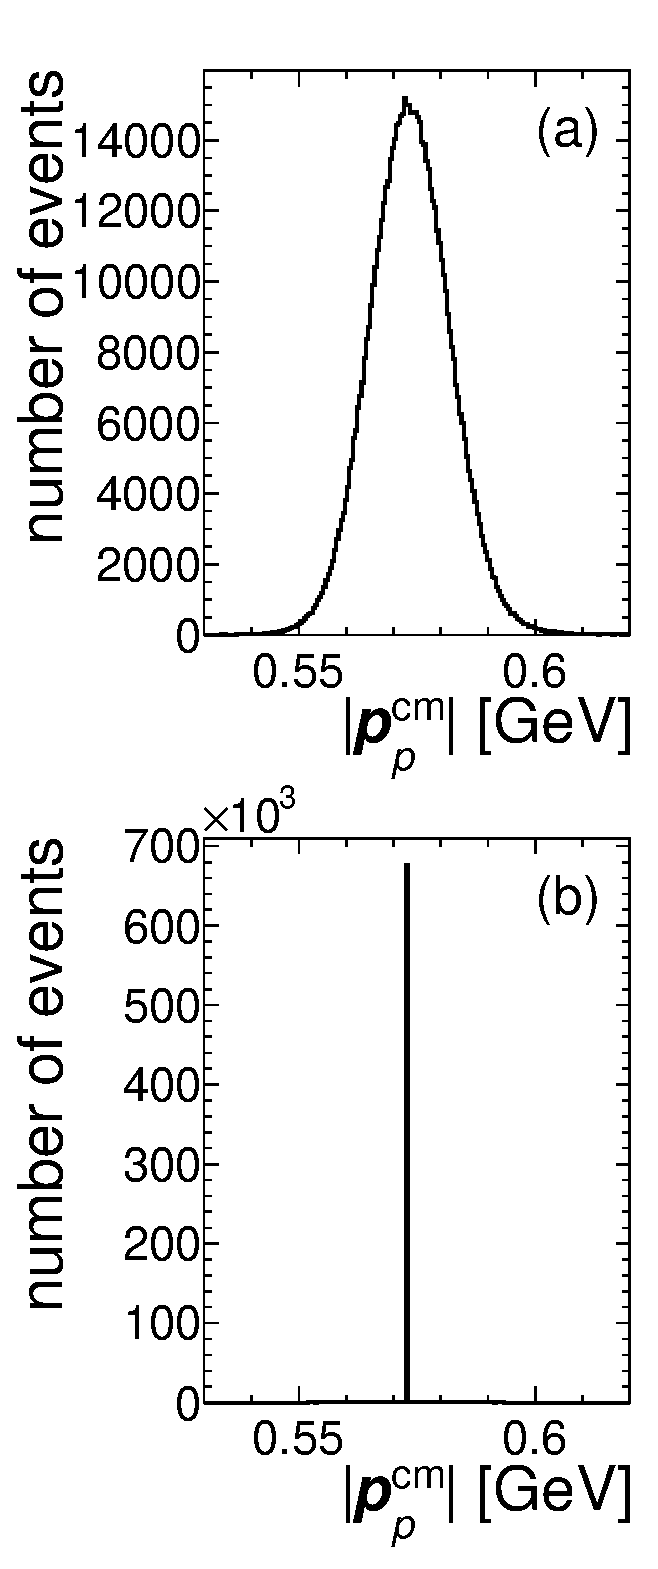
\includegraphics[height=0.7\textheight]{pics/drawMom.eps}
% \hfill
% 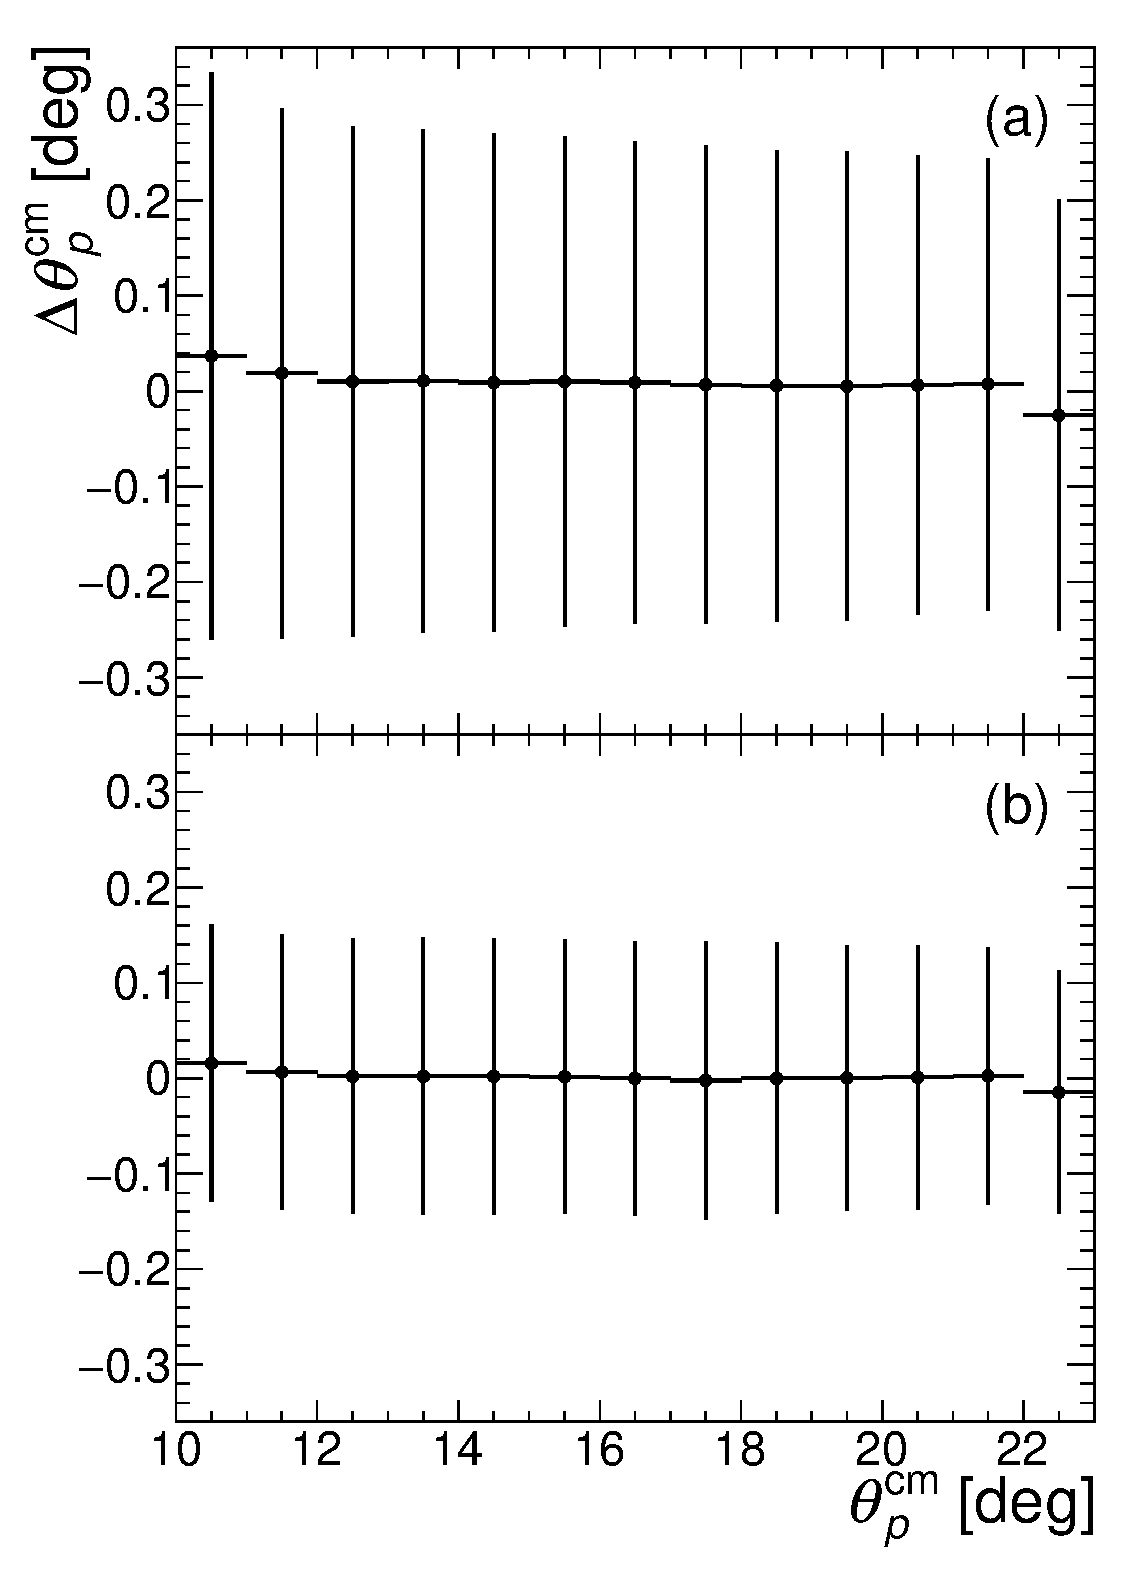
\includegraphics[height=0.7\textheight]{pics/drawTh.eps}
% \hfill
% % \hspace{1em}
% 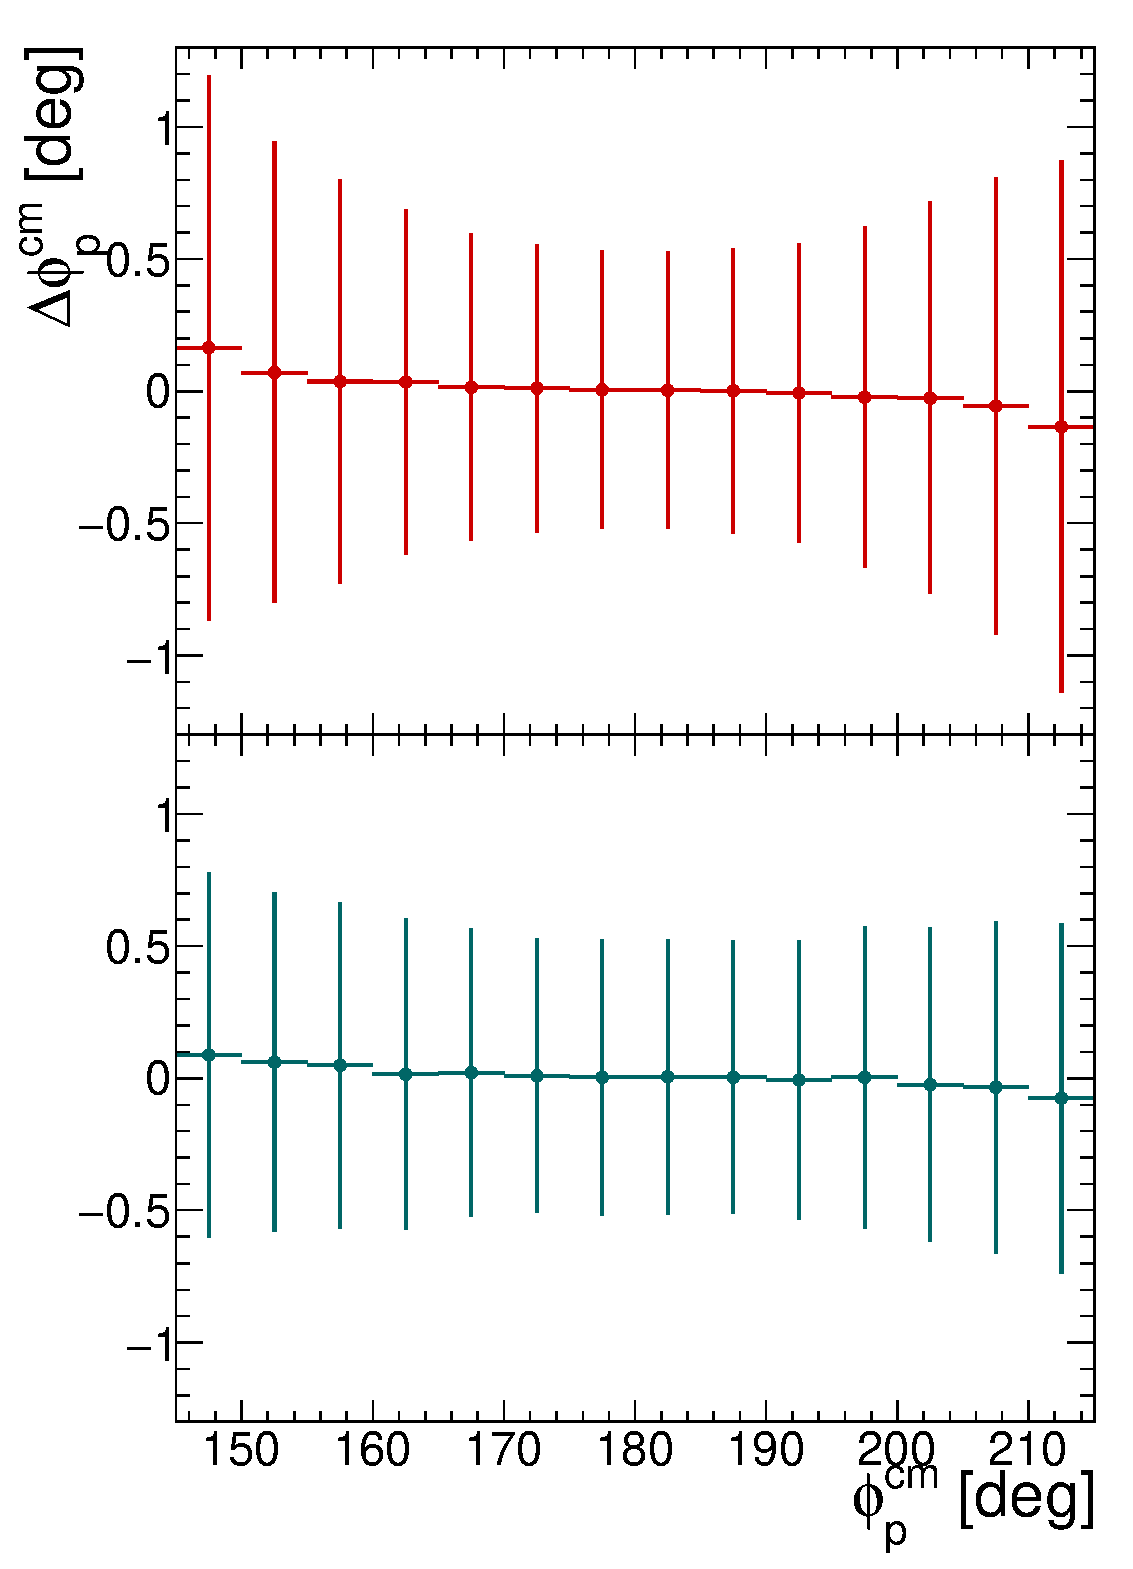
\includegraphics[height=0.7\textheight]{pics/drawPhi.eps}
% \hfill
% \phantom{0}

In order to check the improvement of the momentum precision, about 700\,000 $pp \to pp$ events were simulated and then reconstructed either with or without kinematic constraint \eqref{cons_miss}.
The reconstruction precision for momenta in polar coordinates in center of mass system is shown in fig.~\ref{anke_errs}.
Since $pp \to pp$ is a binary reaction, the condition \eqref{cons_miss} fixes the absolute value of the momentum $|\boldsymbol{p}_p^\mathrm{cm}|$ to the delta function.
Kinematic fitting improves the precision of the polar angle $\theta_p^\mathrm{cm}$ nearly twice.
For the azimuthal angle $\phi_p^\mathrm{cm}$ the improvement not so significant and can be noticed only at the edges of the acceptance.

\section{Conclusion and outlook}
% Outlook

% В ходе работы над кодом для проекта ANKE возникла идея обобщения данного кода и его публикации в открытом доступе для использования всем сообществом.
% Наши ближайшие планы включают в себя рефакторинг и доработку существующего кода, настройку CI/CD для проекта.
% В долгосрочной перспективе видится интересным создание универсального фреймворка для осуществелиния кинематического фита, где с использованием единого интерфейса можно было бы производить кинетический фит не только методом исключения дифференциалов, но и с использованием метода штрафных функций или метода множителей Лагранжа.
During the work on the code for the ANKE project, the idea arose of generalizing this code and publishing it in open access for use by the entire community.
Our immediate plans include refactoring and modifying the existing code, setting up continuous integration and development for the project.
In the long term, it seems interesting to create a universal framework that would use a single interface to perform kinematic fitting not only with the method of elimination of differentials, but also using the penalty function or the Lagrange multiplier method.


% \begin{thebibliography}{00}
% BES-III, % http://iopscience.iop.org/article/10.1088/1674-1137/34/2/009/meta
% CLAS, % https://scholar.google.ru/scholar?cites=6441758058779809394&as_sdt=2005&sciodt=0,5&hl=ru
% CMS. % http://cds.cern.ch/record/926540
\bibitem{BESIII} Y. Liang, H. Rang-Lin et. all, Lagrange multiplier method used in BESIII kinematic fitting, Chinese Physics C, \textbf{34, 2} 204 (2010) \\ URL: \texttt{http://stacks.iop.org/1674-1137/34/i=2/a=009}

\bibitem{CLAS} M.~Williams, D.~Applegate, C.A.~Meyer, Determining Momentum and Energy Corrections for g1c Using Kinematic Fitting, CLAS-NOTE \textbf{04-017} 42 (2004)  \\ URL: \texttt{https://www.jlab.org/Hall-B/notes/clas\_notes04/2004-017.pdf}
% Carnegie Mellon University June 7, 2004

\bibitem{CMS} J.~D'Hondt et all., Fitting of Event Topologies with External Kinematic Constraints in CMS, CMS-NOTE-2006-023, 19 (2006)

\bibitem{anke} ANKE collaboration official web-page\\ URL: \texttt{http://collaborations.fz-juelich.de/ikp/anke/index.shtml}

\bibitem{b1} J.P.~Berge, F.T.~Solmitz, H.D.~Taft, Rev.\ Sci.\ Instr.\ \textbf{32} 538 (1961).
\bibitem{b2} R. Bock, Application of a generalized method of least squares for kinematical analysis of tracks in bubble chambers,       Geneva : CERN, 1960. - 11 p. CERN 60-30 (1960).
\bibitem{b3} G.A. Korn, T.M. Korn, Mathematical handbook for scientists and engineers, McGraw-Hill (1968) 333--335.
\bibitem{b4} P. Avery, KWFIT package\\ URL: \texttt{http://www.phys.ufl.edu/\textasciitilde{}avery/kwfit/}
\bibitem{b5} V.I. Moroz, JINR communications R-1958 (1965)\\ URL: \texttt{http://nu73-73.jinr.ru/\textasciitilde{}cyrkov/MorozJINRCommR1958.pdf}
% \texttt{https://drive.google.com/file/d/1z1hPsccoyXYGA-DT6-7xmeKnYBwPJCS8}
\bibitem{b6} V.S. Kurbatov, I.N. Silin, Nucl. Instrum. Meth. Phys. Res. A 345 (1994) 346--350
% \bibitem{b7} S.N. Dymov et al., Nucl. Instrum. Meth. Phys. Res. A 440 (2000) 431--437
\bibitem{b8} S. Barsov et al., Nucl. Instrum. Meth. Phys. Res. A 462 (2001) 364
\bibitem{b9} V. Komarov et al., Phys. Rev. C 93 (2016) 065206

%НАЙТИ И ПРОЦИТИРОВАТЬ В BIBTEX!
\bibitem{b5} V.I. Moroz, JINR communications R-1958 (1965)\\ URL: \texttt{http://nu73-73.jinr.ru/\textasciitilde{}cyrkov/MorozJINRCommR1958.pdf}
\bibitem{b6} V.S. Kurbatov, I.N. Silin, Nucl. Instrum. Meth. Phys. Res. A 345 (1994) 346--350
\bibitem{b10} S. Dymov et al., FdModule framework\\ URL: \texttt{http://nu73-73.jinr.ru/\textasciitilde{}dymov/FdModule/index.html}
\bibitem{fum_1st} S.N. Sokolov and I.N. Silin, Preprint JINR, D-810, Dubna(1961)

% % Zainon, R., Butler, A. P. H., Cook, N. J., Butzer, J. S., Schleich, N., de Ruiter, N., Tlustos, L., Clark, M. J., Heinz, R. & Butler, P. H. (2010). Construction and operation of the MARS-CT scanner,
% % Internetworking Indonesia Journal 2(1): 3–10.
% \bibitem{mars}
% R.~Zainon, A.P.H.~Butler \textit{et al.}, Internetworking Indonesia Journal \textbf{2(1)}, 3--10 (2010).
%
% \bibitem{dicom}
% DICOM standard official site, available at http://dicom.nema.org/standard.html.
%
% \bibitem{turbel}
% H.~Turbell, \textit{Cone-beam reconstruction using filtered back-projection}, Link\"oping University Electronic Press, 189 (2001).
% %
% % and use \bibitem to create references.
% \bibitem{trends}
% I.~Scholl, T.~Aach, T.M.~Deserno \textit{et al.}, Comput.\ Sci.\ Res.\ Dev.\ \textbf{26}, 5--13 (2011).
%
% \bibitem{Roobot}
% C.A.~Roobottom, G.~Mitchell, G.~Morgan-Hughes, Clin.\ Radiol.\ \textbf{65 (11)}, 859--67 (2010).
%
% \bibitem{popularCT}
% T.~Hiroyasu, Y.~Minamitani, M.~Yoshimi, M.~Miki, WORLDCOMP'11 \textbf{2011-MRS-84 (5)} (2011).
%
% \bibitem{hierarhCT}
% S.~Xiao, Y.~Bresler, D.C.~Munson, Proceedings 2003 International Conference on Image Processing \textbf{2}, II–819–22 (2003).
%
% \bibitem{77}
% L.~Feldkamp, L.~Davis, J.~Kress, Journal of the Optical Society of America A \textbf{1(6)}, 612--619 (1984).
%
% \bibitem{bigObserve}
% A.~Belle, BioMed Research International \textbf{2015}, 16 (2015).
%
% % \bibitem{Scherl}
% % H.~Scherl, \textit{Evaluation of State-of-the-Art Hardware Architectures for Fast Cone-Beam CT Reconstruction} (Springer Fachmedien Wiesbaden GmbH, Wiesbaden, 2011) XX, 138
% %
% % \bibitem{Yu}
% % L.~Zhou, J.~Chang, Medical Physics \textbf{39} 4000 (2012)
% %
% % \bibitem{Ramani}
% % S.~Ramani, J.A.~Fessler, IEEE Transactions on Medical Imaging, \textbf{31 (3)}, 677 (2012)
% %
% % \bibitem{Yan}
% % G.~Yan, S.~Zhu, Y.~Dai, C.~Qin, Journal of X-Ray Science and Technology \textbf{16 (626)} 225--234 (2008).
%
% \bibitem{76}
% B.~Meng, G.~Pratx, L.~Xing, Med.\ Phys.\ \textbf{38(12)} 6603--6609 (2011).
%
% % \bibitem{77}
% % C.F.~Mackenzie, P.~Hu, A.~Sen et al., AMIA Annual Symposium Proceedings \textbf{2008} 318--322 (2008)
%
% \bibitem{chinese}
% C.-T.~Yang, C.-T.~Kuo, W.-H.~Hsu, W.-C. Shih, Proceedings of the 7th international conference on Advances in Grid and Pervasive Computing \textbf{7296}, 338--349 (2012).
%
% \bibitem{HDFS} HDFS documentation, available at http://hadoop.apache.org/docs/current/hadoop-project-dist/hadoop-hdfs/HdfsDesign.html.

%###################################################################################
% \bibitem{RefJ}
% Format for Journal Reference
% Journal Author, Journal \textbf{Volume}, page numbers (year)
% Format for books
% \bibitem{RefB}
% Book Author, \textit{Book title} (Publisher, place, year) page numbers
% etc
\end{thebibliography}

% \bibliographystyle{webofc}
\bibliography{biblio}

\end{document}
